\documentclass{article}
\usepackage{ee105}

%% Makes figure labels bold
\usepackage[labelfont=bf]{caption}

\begin{document}
\thispagestyle{plain}

\tutorial{HP 4145B/4155A/4155C Parameter Analyzer}

\tableofcontents

\section{Introduction}

The HP 4145B/4155A/4155C is a parameter analyzer. It can be used to apply test signals (voltages or currents) to one or more nodes of a circuit, then measure the voltages and currents at other nodes in the circuit. What makes the parameter analyzer particularly useful is that it can sweep a test voltage across hundreds of values in a matter of seconds. You can think of its capabilities like those of a DC analysis in SPICE.

\section{The Hardware Interface}

The hardware interface to the HP 4145B/4155A/4155C is a metallic box (called a test fixture) located at every lab station. Inside the test fixture, you'll notice a socket, many numbered slots, and eight labeled terminals: 4 SMU, 2 VS, and 2 VM (newer models have more terminals, but all models have at least these eight). The SMU is the most flexible terminal: it can be used to apply or measure a current or a voltage. The VS can act only as a voltage source, and the VM can act only as a voltmeter. For any measurement you're conducting having fewer than five nodes, you should use the SMU terminals for all of the nodes since they provide the most functionality. Figure \ref{testold} shows the old test fixture and Figure \ref{testnew} shows the new test fixture. SMU terminals are labeled with red, VS with blue, VM with black, and ground with green. Note that the HP 16147 test fixture has two numbering schemes for the SMU terminals---use the the numbering scheme with black numbers on a white background (as labeled in Figure \ref{testnew}).

\begin{figure}[!htb]
  \centering
  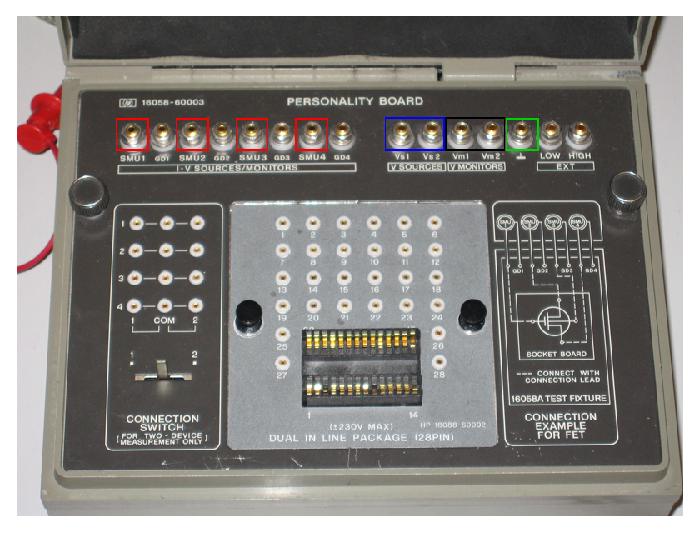
\includegraphics{testold.eps}
  \caption{HP 16058 test fixture}
  \label{testold}
\end{figure}

\begin{figure}[!htb]
  \centering
  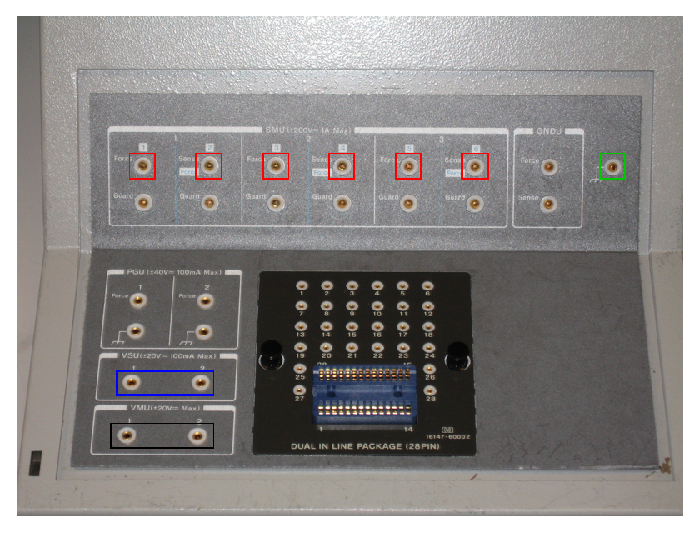
\includegraphics{testnew.eps}
  \caption{HP 16147 test fixture}
  \label{testnew}
\end{figure}

When using the HP 4145B/4155A/4155C, you can either connect a pin to the ground terminal in the test fixture or you can connect it to an SMU or VS and set the SMU/VS to supply 0V. According to the test fixture documentation, the ground terminals are just connected to the chassis of the test fixture, so using the ground terminal can mean a noisy ground. For best results (in particular with small signals or sensitive circuitry), you should use an SMU or VS for ground.

In order to actually hook up a circuit to the HP 4145B/4155A/4155C, you'll need special cables provided by your TA. These are extremely expensive (\$70 a piece!), so be careful not to break or lose them. Build your circuit on the breadboard provided in lab, then use the special cables to connect nodes in your circuit to SMU, VS, and VM terminals depending on the functionality you need at each node.

\section{The Software Interface}

Before using the software interface, you must turn on the HP 4145B/4155A/4155C. There is a power button in the lower left hand corner (it may take 20-30 seconds for the machine to start). The software to interface with the HP 4145B/4155A/4155C is only installed on half of the computers in the lab, since there are two computers per lab station but only one set of lab equipment. Generally, the computer located closer to the HP 4145B/4155A/4155C (the one to the left of the machine) is the computer with the software. Computers that have the software installed are labeled ``Metrics Installed'' as well.

\begin{enumerate}
  \item Start ICS Metrics. Click \textit{Start} $\rightarrow$ \textit{Programs} $\rightarrow$ \textit{Metrics} $\rightarrow$ \textit{ICS}. You may get an error, but just click \textit{OK} to ignore it.

  \item Click \textit{Instruments} $\rightarrow$ \textit{Select Instrument...} (or the icon in Figure \ref{instrument}). You should see a list of ``Available'' instruments on the left side of the window. Select the instrument that is installed at your lab station (select HP4145 for the HP 4145 and HP4155-6 for the HP 4155A/4155C). Click \textit{Connect} and the device should be listed under ``Selected''. Click \textit{OK} to exit this window.

\begin{figure}[!htb]
  \centering
  
\includegraphics{instrument.eps}
  \caption{Icon for selecting an instrument}
  \label{instrument}
\end{figure}

  \item Click \textit{Measure} $\rightarrow$ \textit{Edit Setup...} (or the icon in Figure \ref{setup}) to open the Setup Editor. Click \textit{New} to create a new setup and give it a name (any name is fine).

\begin{figure}[!htb]
  \centering
  
\includegraphics{setup.eps}
  \caption{Icon for setting up a measurement}
  \label{setup}
\end{figure}

  \begin{enumerate}
    \item You should now see a schematic of a MOSFET with blue squares at each terminal. Click \textit{Device} to pick a different device. \textbf{Note that the device shown is only to help you connect terminals. It does not change anything other than the number of terminals available.} After selecting the device, click \textit{OK}. If you picked a different device, the schematic will change and the number of terminals will change.
    \item Now you must assign an SMU, VM, or VS to each of the terminals in the diagram. This interface allows you to specify how the circuit is connected to the hardware interface. Click \textit{Source Units}. A new window will come up with all of the SMU, VM, and VS terminals of the hardware interface available for you to select. Click the source unit you want to assign, then click on one of the terminals to assign that source unit to that terminal. The schematic will change to show you which SMU, VS, or VM you've assigned to which terminal.
    \item You can now assign stimuli and measurements to the terminals that you've labeled. For each terminal, click on the icon next to the label and a new window will come up showing all of the available measurement and stimulus options. For the VS and VM terminals, you'll only be able to apply or measure a voltage, respectively. For SMU terminals, you can choose to have either a voltage of current stimulus in the upper left hand corner. You can choose to measure voltage or current in the upper middle of the window. Finally, you can select the actual values for the stimulus in the middle portion of the window. (\textit{Note: If you want to measure the voltage at a terminal without applying a signal, you can apply a current stimulus of amplitude zero, which won't change your circuit}.)
    \item There are four primary ways you can set a stimulus (current or voltage). The first is just a constant value. You won't be using this much, since constant measurements are easy to do with a DC power supply and multimeter and don't require something as complex as the HP 4145B/4155A/4155C. You can also set a node to common, which is ground (this is exactly equivalent to setting it to a constant value of 0V). You'll always have one ground node in your circuit. Finally, the interesting options are stepping and sweeping values.
      \begin{itemize}
	\item Stepping a value causes a measurement to occur at every voltage you select. You can set a starting voltage, a stopping voltage, and how many points you want to test.
	\item Sweeping a value causes a measurement sweep to occur at every stepped voltage. For example, you could step a voltage $V_1$ from \unit{0}{\volt} to \unit{5}{\volt} in increments of \unit{1}{\volt} and sweep another voltage $V_2$ from \unit{0}{\volt} to \unit{5}{\volt} in increments of \unit{0.1}{\volt}. This would cause the HP 4145B/4155A/4155C to set $V_1=\unit{0}{\volt}$, then sweep $V_2$, then set $V_1=\unit{1}{\volt}$, then sweep $V_2$ again, etc. until $V_1=\unit{5}{\volt}$ and $V_2$ is swept for the last time. Using this feature, you can obtain a family of curves, such as the I-V curves of a transistor.
      \end{itemize}
      Note that when stepping and sweeping values, we often tell ICS Metrics to use one more data point than you'd expect. For example, when stepping from \unit{0}{\volt} to \unit{5}{\volt}, we would use 6 data points rather than 5 in order to achieve a step size of \unit{1}{\volt}. Similarly, when sweeping a voltage from \unit{0}{\volt} to \unit{5}{\volt}, we would use 101 data points rather than 100 in order to get a step size of an even \unit{0.05}{\volt}.
      When you're done assigning SMU, VS, and VM terminals and associated measurements, click \textit{Done} to close the Setup Editor.
  \end{enumerate}
  \item All that's left is to run the measurements you've done. In order to do this, click \textit{Measure} $\rightarrow$ \textit{Measure...}. This will bring up a panel on the right side of the screen. Click the button labeled \textit{Single}, which has the appearance of a right arrowhead. Once the measurement is completed, a new window will come up showing all of the data in a spreadsheet (the spreadsheet may be minimized, so click the restore icon to make it show).

\begin{figure}[!htb]
  \centering
  
\includegraphics{measure.eps}
  \caption{Icon for running a measurement}
  \label{measure}
\end{figure}

  \item Now that you have measurement data, you can use ICS to create a plot. Click \textit{Window} $\rightarrow$ \textit{New Plot...} (or the icon in Figure \ref{plot}). A new window will come up allowing you to choose which values in the spreadsheet should be used on the $x$ and $y$ axes. Make the appropriate choices (you may also select linear or log scales), then click \textit{Done} to close the window. You should be able to see the plot you created.

\begin{figure}[!htb]
  \centering
  
\includegraphics{plot.eps}
  \caption{Icon for plotting measurement results}
  \label{plot}
\end{figure}

    \begin{itemize}
      \item If you want to print the plot directly from ICS, \textbf{do not print without setting a white background first}. You will waste an immense amount of ink if you do not set a white background. In order to set a white background, click \textit{Setup} $\rightarrow$ \textit{Colors...} and select the radio button labeled \textit{Monochrome}. Click \textit{Done} and you'll see the plot is now black with a white background.
      \item You can also use Microsoft Excel to make plots. This can be useful because of Excel's ability to fit curves. See the section on Microsoft Excel for details on plotting and fitting data in Excel.
    \end{itemize}
\end{enumerate}

\section{Microsoft Excel}

\begin{enumerate}
  \item Click \textit{Start} $\rightarrow$ \textit{Programs} $\rightarrow$ \textit{Microsoft Office} $\rightarrow$ \textit{Microsoft Office Excel 2003}. A window titled ``Windows Installer'' may come up. If it does, click \textit{Cancel} and Excel should start.
  \item Select your data in ICS by dragging your mouse over all of the data you measured. Copy it using \textit{ctrl}+\textit{c} and paste it into Excel using \textit{ctrl}+\textit{v}.
  \item Your data will probably contain scientific notation suffixes such as `m' and `u'. Excel doesn't understand these suffixes, so you have to use the find and replace feature in Excel to remove these. Click \textit{Edit} $\rightarrow$ \textit{Replace...}. In the box labeled ``Find what:'', enter `m'. In the ``Replace with:'' box, enter `e--3'. Click \textit{Replace All}. Do the same for `n' and `u' (using `e--9' and `e--6' as the replacements, respectively).
  \item Click \textit{Insert} $\rightarrow$ \textit{Chart}. Under ``Chart type'', select \textit{XY (Scatter)}. Under ``Chart sub-type'', select the second option (the description is ``Scatter with data points connected by smooth lines.''). Click \textit{Next}.
  \item Select the \textit{Series} tab. Select the appropriate ``X Values'' and ``Y Values'' in this window (use Microsoft Excel's help feature if you need help doing this), then click \textit{Next}.
  \item Label your chart and the $x$ and $y$ axes in this window. You can also include a legend if you have more than one curve on the graph.
  \item Click \textit{Next}. Choose whether you want the chart to be a new sheet or an object in the current sheet. Click \textit{Finish}.
  \item Your chart should now be visible. To add a trendline, right-click the curve you want to add the trendline too, then click \textit{Add Trendline...}. Select the type of trendline to use (most likely you'll want a linear trendline). Select the \textit{Options} tab and click the checkbox labeled ``Display equation on chart''. Click \textit{OK}.
  \item The trendline and associated equation will be displayed on the chart. You can use the equation to get the slope of the line and the $x$--intercept, which are often related to device parameters.
\end{enumerate}

\end{document}
